\documentclass[letterpaper, 12 pt, conference]{ieeeconf} 
\IEEEoverridecommandlockouts                              
\overrideIEEEmargins
\usepackage{setspace}
\usepackage{hyperref}
\hypersetup{
    colorlinks=true,
    urlcolor=blue,
    }

\urlstyle{same}
\usepackage{wrapfig}




% The following packages can be found on http:\\www.ctan.org
\usepackage{graphics} % for pdf, bitmapped graphics files
%\usepackage{epsfig} % for postscript graphics files
%\usepackage{mathptmx} % assumes new font selection scheme installed
\usepackage{times} % assumes new font selection scheme installed
%\usepackage{amsmath} % assumes amsmath package installed
%\usepackage{amssymb}  % assumes amsmath package installed
\usepackage{graphicx}

\begin{document}

\thispagestyle{empty}
\pagestyle{empty}

\begin{titlepage}
    \begin{center}
        \vspace*{2.5cm}
 
        \textbf{Feedback Dashboarding Tool}
 
        \vspace{0.5cm}
         Thesis Subtitle
 
         \vfill
        
 
        \textbf{Genevieve Couture}
        200426387 grc839@uregina.ca
 
        \textbf{Payton Gilbertson}
        200248472 gilbertp@uregina.ca
 
        \textbf{Liam Gulak}
        200393578 lgq292@uregina.ca
 
        \textbf{Yunseok Kim}
        200434122 yjk172@uregina.ca
 
        \textbf{Zachary Huber}
        200408160 zeh434@uregina.ca
 
        \vspace{1.5cm}  
        CS 476 Project Report
             
        \vspace{0.8cm}
      
             
        University of Regina\\
        March 21, 2023
             
    \end{center}
 \end{titlepage}


%%%%%%%%%%%%%%%%%%% BODY %%%%%%%%%%%%%%%%%%%%%%%%%%%%%%%%%%%%%%%%%%%%%%%%%%%%%%%%


\doublespacing 
\onecolumn

\section{Problem Definition}
\subsection{outline the problem requirements and include the application domain and motivations of your project (1 page).}

Business and product owners want meaningful feedback from their customers to assist in their growth and success. It can be difficult to collect this information without onsite hardware and processing the data provided can be a timely task. As with many forms of customer engagement and ratings, customers can be unwilling to participate in traditional methods of feedback if too many steps are required, so the data collected will not be an accurate portrayal of opinions.

In order to solve this problem, we have created a web application that allows for customers to provide their feedback in a simplistic way, and displays this information for businesses or owners in a way that it simple to understand without the need for onsite hardware. By allowing the customer to interact with a site that is not cumbersome, and can be done from the convenience of their smart phone, many more customers will be willing to submit their thoughts and opinions.










\newpage    
\section{Application Benefits}
\subsection{what are the benefits of your application when compared to existing systems. Choose two systems only and include their references (2 pages).}

Our application is a simple tool for conducting self-administered surveys. Our users can log into their profiles to view customer feedback to improve their businesses. QR codes can be generated for wide distribution and quick access. SurveyMonkey (https://www.surveymonkey.com/) and QuestionPro (https://www.questionpro.com/) are comparable existing systems. Some benefits of our application are that the users can received unlimited number of responses for their surveys without cost and all features to create the surveys are free as well. Our application does not have many templates and complicated tools that may negatively impact loading time. Respondents do not need to create an account to respond to surveys. 

\textbf{discuss survey monkey differences}

\textbf{discuss questionpro differences}


\newpage
\section{Requirements Elicitation and Specification}
\subsection{Functional requirements list (only the ones that you have implemented) for each user role (two exactly). Name each requirement and explain it briefly.}

\textbf{Feedback Gatherer}
\begin{enumerate}
   \item \textbf{Register:} Feedback gatherer creates an account by entering the required information
   \item \textbf{Create Survey:} Feedback gatherer creates a survey by entering questions and selecting type of responses
   \item \textbf{View QR Code:} Feedback gatherer views the generated QR code for the survey
   \item \textbf{Delete Survey:} Feedback gatherer deletes a survey that is no longer required
   \item \textbf{View Statistics and Responses:} Feedback gatherer views statistics and responses of a selected survey
\end{enumerate}

\textbf{Respondent}
\begin{enumerate}
   \item \textbf{Scan QR Code:} Respondent scans the QR code to view the survey
   \item \textbf{Enter Responses:} Respondent enters responses to the survey questions
   \item \textbf{Submit Response:} Respondent submits responses to the survey questions
\end{enumerate}

%\newpage

\subsection{For each user role, provide the use case diagram with all the use cases and actors.}
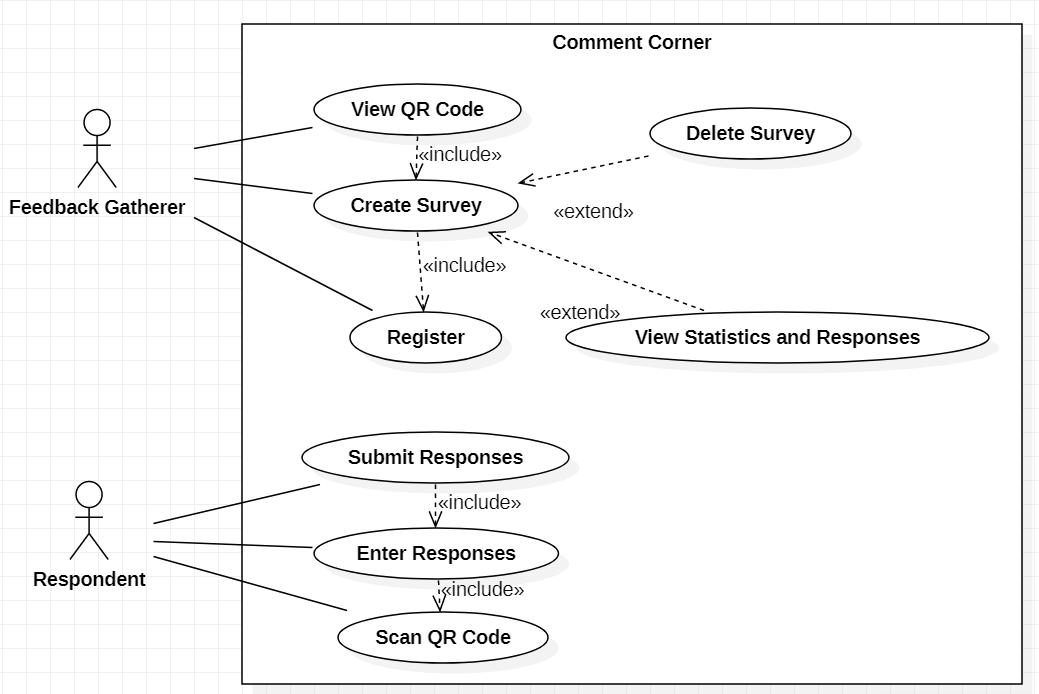
\includegraphics[width=0.70\textwidth]{caseDiagram.png}

\newpage
\subsection{Describe in detail two use cases using the activity diagram. Choose the most complex use cases.}
\begin{enumerate}
    \item The feedback gatherer can create a survey after registering. The feedback gatherer has the option to delete an existing survey or view statistics and responses to an existing survey. After creating a survey, the feedback gatherer can view the QR code to administer the created survey.
    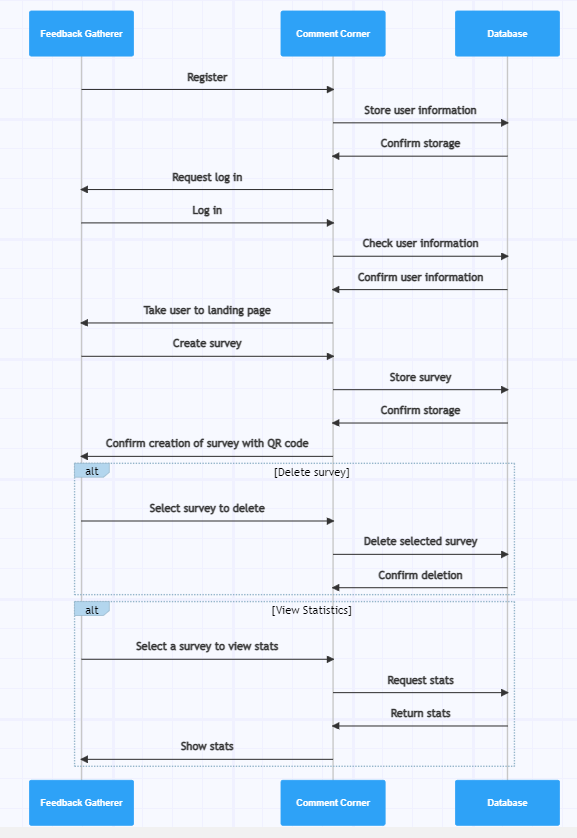
\includegraphics[width=0.70\textwidth]{feedbackGatherer.png}
\newpage
    \item The respondent can scan the QR code to take a survey created by a feedback gatherer. The respondent enters responses to the survey and submit the responses.
    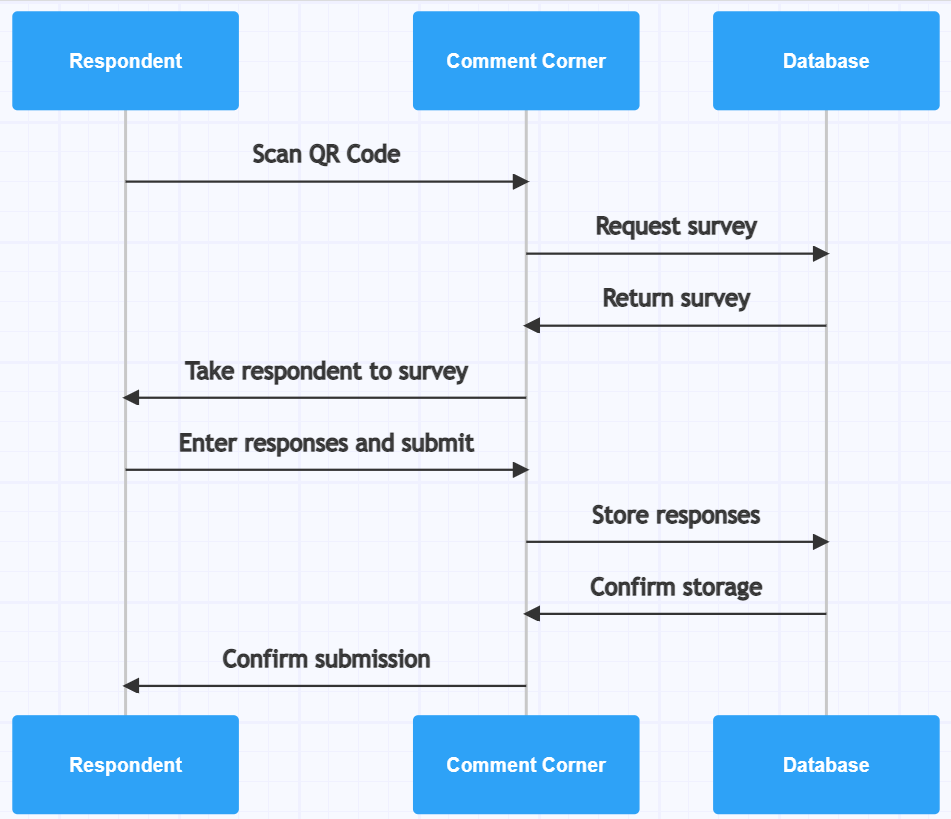
\includegraphics[width=0.70\textwidth]{respondent.png}
\end{enumerate}

\subsection{Software qualities: Correctness, Time-efficiency and Robustness. Include at least two concrete examples for each quality for each user role. The sign-in and sign-up use cases are excluded from the examples.}

\textbf{Correctness:}
\begin{enumerate}
    \item[] Feedback Gatherer:
    \begin{itemize}
        \item A survey correctly displays the questions and answer choices entered by the feedback gatherer during creation. 
        \item Accurate statistics for a survey are shown to the feedback gatherer.
    \end{itemize}
    \item[] Respondent:
    \begin{itemize}
        \item Scanning the QR code takes the respondent to the correct survey.
        \item Responses to a survey are saved correctly.
    \end{itemize}
\end{enumerate}

\textbf{Time Efficiency:}
\begin{enumerate}
    \item[] Feedback Gatherer:
    \begin{itemize}
        \item  When a feedback gatherer creates the survey, the QR code for the survey is created in a timely manner.
        \item When responses to a survey are submitted, they are available for view by the feedback gatherer in a timely manner.
    \end{itemize}
    \item[] Respondent:
    \begin{itemize}
        \item A respondent is taken to the survey in a timely manner after scanning a QR code for a survey.
        \item A respondent is given a confirmation in a timely manner after submitting a survey.
    \end{itemize}
\end{enumerate}


\textbf{Robustness:}
\begin{enumerate}
    \item[] Feedback Gatherer:
    \begin{itemize}
        \item  If a feedback gatherer attempts to submit a blank survey, submission is denied with a warning.
        \item If a feedback gatherer forgets to select a type of answer to a question, submission is denied with a warning.
    \end{itemize}
    \item[] Respondent:
    \begin{itemize}
        \item If a respondent attempts to submit a survey with one or more unanswered questions, submission is denied and unanswered questions are marked.
        \item If a respondent attempts to exit the survey after answering one or more questions, a warning is shown.
    \end{itemize}
\end{enumerate}


\section{Top-level and Low-level Software Design}
\subsection{Provide the MVC architecture according to the selected Web frame- work. Also, describe at least three benefits of MVC for your application.}
\subsection{Observer and Factory design patterns. Explain in detail the usability of these two patterns for your specific application. Include the complete class diagram for each pattern. Also provide the algorithms corresponding to the pattern’s important methods. For each class, provide the data types of the attributes and prototypes of the methods.}
\subsection{Provide the class diagram of the whole system by incorporating the two design patterns.}

\section{Software Construction}
\subsection{Submit the screenshot of the entire structure of the code within the web framework.}
\subsection{Deployment diagram regarding the hardware configuration of the code. Indicate the supported Web browsers, the application/Web servers and the database solution.}
\subsection{Screenshots of all table contents of the system data.}
\subsection{GitHub link of the entire program. All students must contribute equally to the programming part. The commit log of each student will be checked within GitHub. Website builders, such as Wordpress, are not allowed.}
\url{https://github.com/zachary-huber/feedback-app}

\subsection{Link of your Web-based application. The application should be accessible online and runnable.}
\url{https://www.viewnote.app/}

\section{Technical Documentation}
\subsection{List of programming languages.}
\begin{enumerate}
   \item Javascript
   \item HTML
   \item CSS
   \item PHP
\end{enumerate}

\subsection{List of reused algorithms and programs. Include their sources.}
\begin{enumerate}
   \item thing
   \begin{description}
     \item description
   \end{description}
   \item thing
\end{enumerate}

\subsection{List of software tools and environments. Provide briefly their benefits specifically for your application.}
\begin{enumerate}
   \item React
   \begin{description}
     \item description
   \end{description}
   \item Django
\end{enumerate}

\section{Acceptance Testing: select test cases for both user roles. The sign-in and sign-up are excluded from testing.}
\subsection{Correctness testing using four test cases (screenshots of both inputs and out- puts).}
\subsection{Robustness testing using four test cases (screenshots of both inputs and out- puts).}
\subsection{Time-efficiency testing of two functions (with screenshots). Indicate the method you used to measure the time.}



\addtolength{\textheight}{-12cm}


%%%%%%%%%%%%%%%%%%%%%%%%%%%%%%%%%%%%%%%%%%%%%%%%%%%%%%%%%%%%%%%%%%%%%%%%%%%%%%%%



%%%%%%%%%%%%%%%%%%%%%%%%%%%%%%%%%%%%%%%%%%%%%%%%%%%%%%%%%%%%%%%%%%%%%%%%%%%%%%%%


%%%%%%%%%%%%%%%%%%%%%%%%%%%%%%%%%%%%%%%%%%%%%%%%%%%%%%%%%%%%%%%%%%%%%%%%%%%%%%%%

\newpage


\begin{thebibliography}{99}

\bibitem{young-1964} G. O. Young, Synthetic structure of industrial plastics (Book style with paper title and editor), 	in Plastics, 2nd ed. vol. 3, J. Peters, Ed.  New York: McGraw-Hill, 1964, pp. 15Ð64.
\bibitem{chen-1993} W.-K. Chen, Linear Networks and Systems (Book style).	Belmont, CA: Wadsworth, 1993, pp. 123Ð135.
\bibitem{poor-1985} H. Poor, An Introduction to Signal Detection and Estimation.   New York: Springer-Verlag, 1985, ch. 4.

\bibitem{uofr} "Home", University of Regina, 2022. [Online]. Available: https://www.uregina.ca/. [Accessed: 06- Apr- 2022].

\end{thebibliography}




\end{document}
